\documentclass[10pt, twocolumn]{article}
\usepackage[margin=0.48in]{geometry}
\usepackage{graphicx}
\usepackage{booktabs}
\usepackage{float}
\usepackage{amsmath}
\usepackage[font=small,labelfont=bf]{caption}

\title{\vspace{-15mm}\Large\textbf{Milestone 2 Report}}
\author{SCIPER 392412 $\cdot$ 373176 $\cdot$ 398388}
\date{}

\begin{document}

\setlength{\abovedisplayskip}{2pt}
\setlength{\belowdisplayskip}{2pt}
\setlength{\abovedisplayshortskip}{1pt}
\setlength{\belowdisplayshortskip}{1pt}

\maketitle

\section{Introduction}
Same as Milestone 1, with the Gaming and Mental Health dataset, we have 2,000 samples total, keeping 1,600 for training and 400 for testing. We want to predict two targets. First, we predict the continuous addiction score (0 to 10). Second, we classify the general addiction level into Low, Medium, or High.

In this milestone, we implement a Multi-Layer Perceptron (MLP) from scratch for both tasks. We also implement K-Means clustering for classification. It was very interesting to compare a neural network against clustering.

\section{Dataset and Preprocessing}
We prepared the data by applying standard z-score normalisation. We calculated means and standard deviations from the training set only. To avoid data leakage, we split our 1,600 training samples into an 80/20 train/validation split. This leaves 1,280 samples for training and 320 for local tuning.

While doing this split, we discovered a severe class imbalance in the training labels. Class 0 (Low) has 1,103 samples (68.9\%), Class 1 (Medium) has 446 samples (27.9\%), and Class 2 (High) has only 51 samples (3.2\%). This imbalance makes classification quite challenging.

\begin{figure*}[t!]
    \centering
    \begin{minipage}{0.32\textwidth}
        \centering
        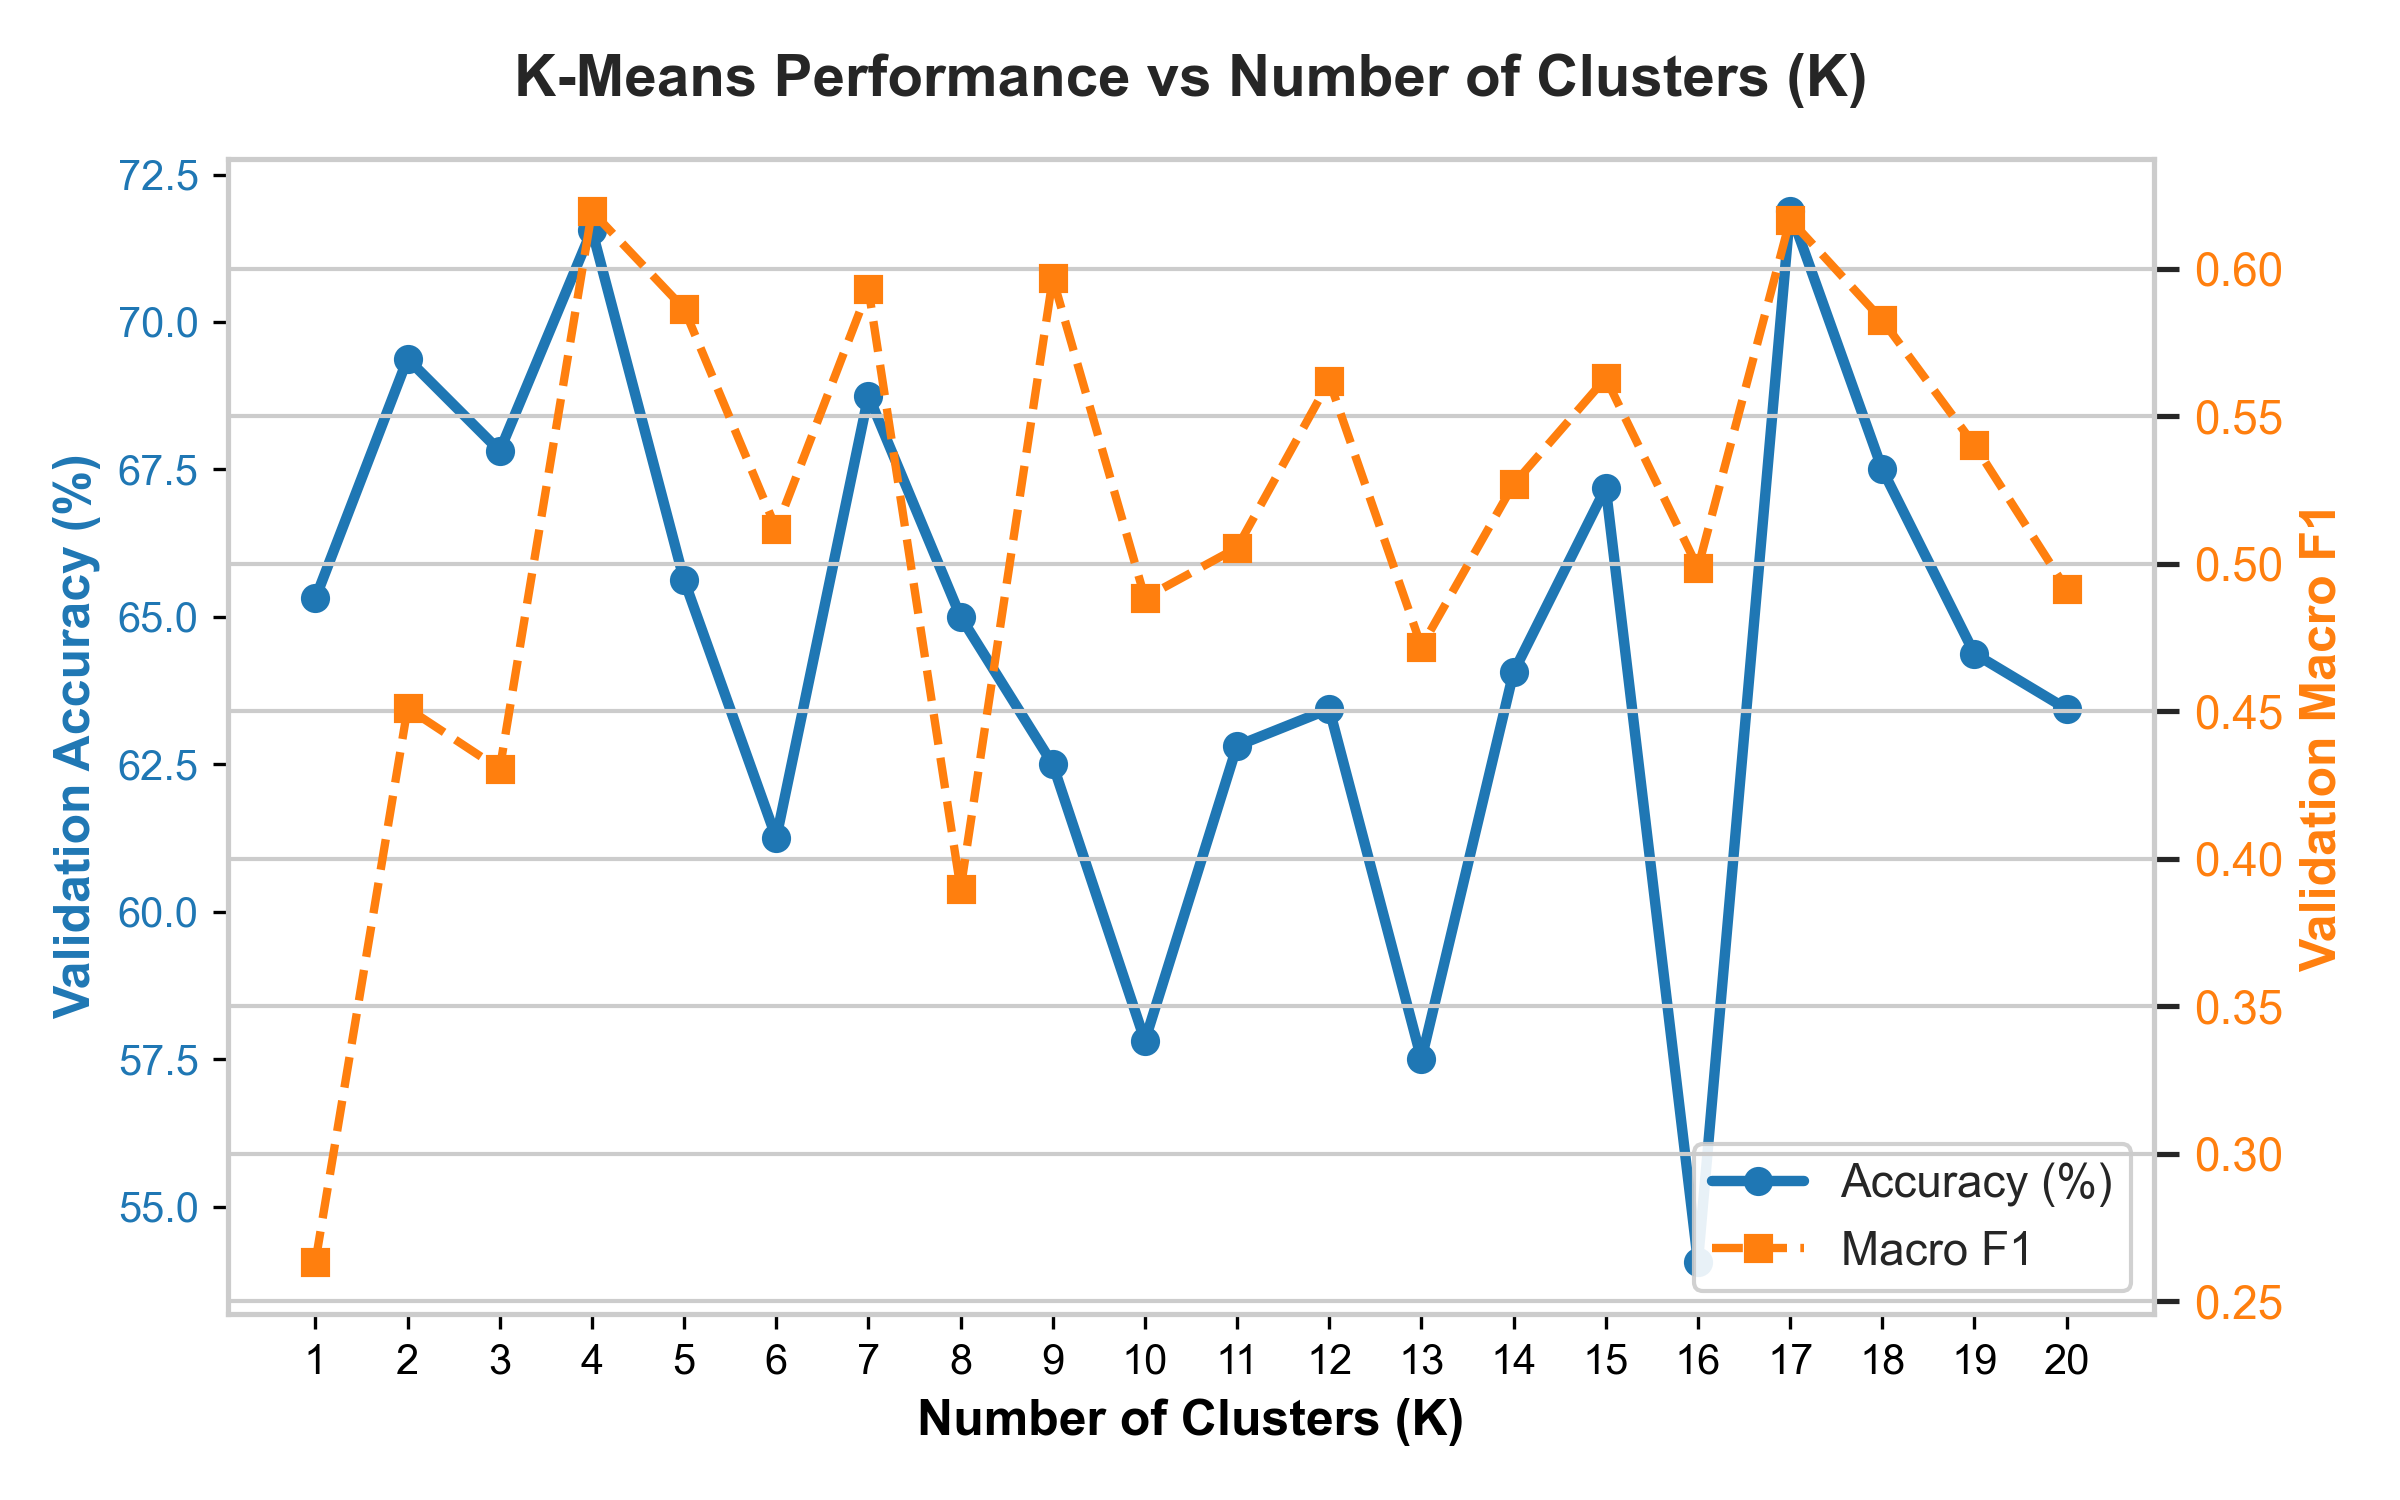
\includegraphics[width=0.96\linewidth]{kmeans_sweep.png}
        \caption{K-Means validation metrics vs. K.}
        \label{fig:kmeans}
    \end{minipage}\hfill
    \begin{minipage}{0.32\textwidth}
        \centering
        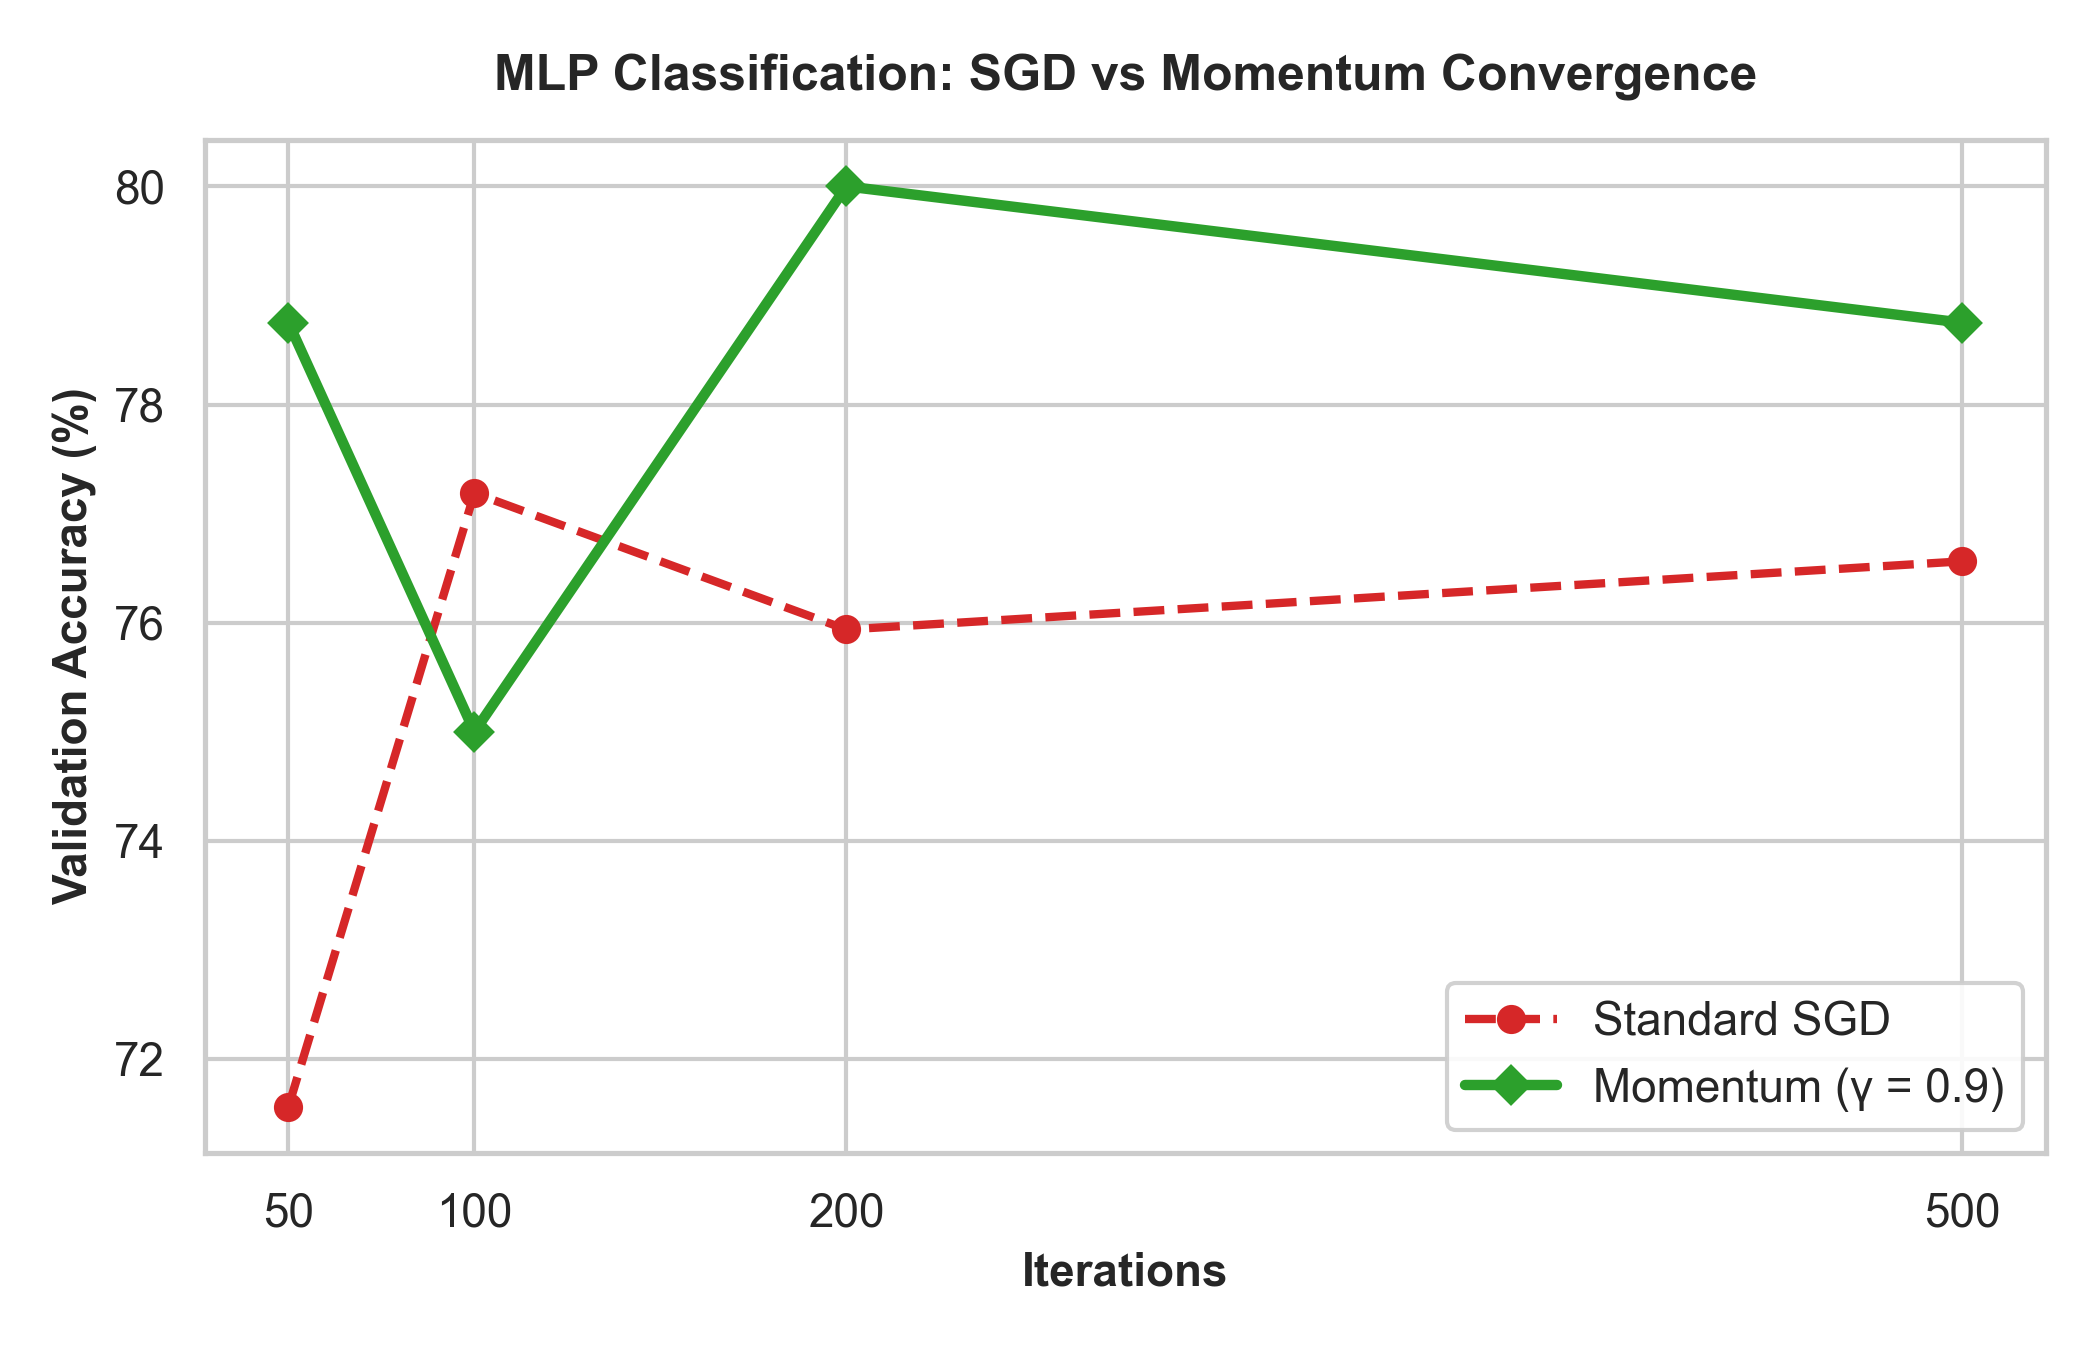
\includegraphics[width=0.96\linewidth]{mlp_class_comparison.png}
        \caption{MLP Classification: SGD vs Momentum.}
        \label{fig:mlp_class}
    \end{minipage}\hfill
    \begin{minipage}{0.32\textwidth}
        \centering
        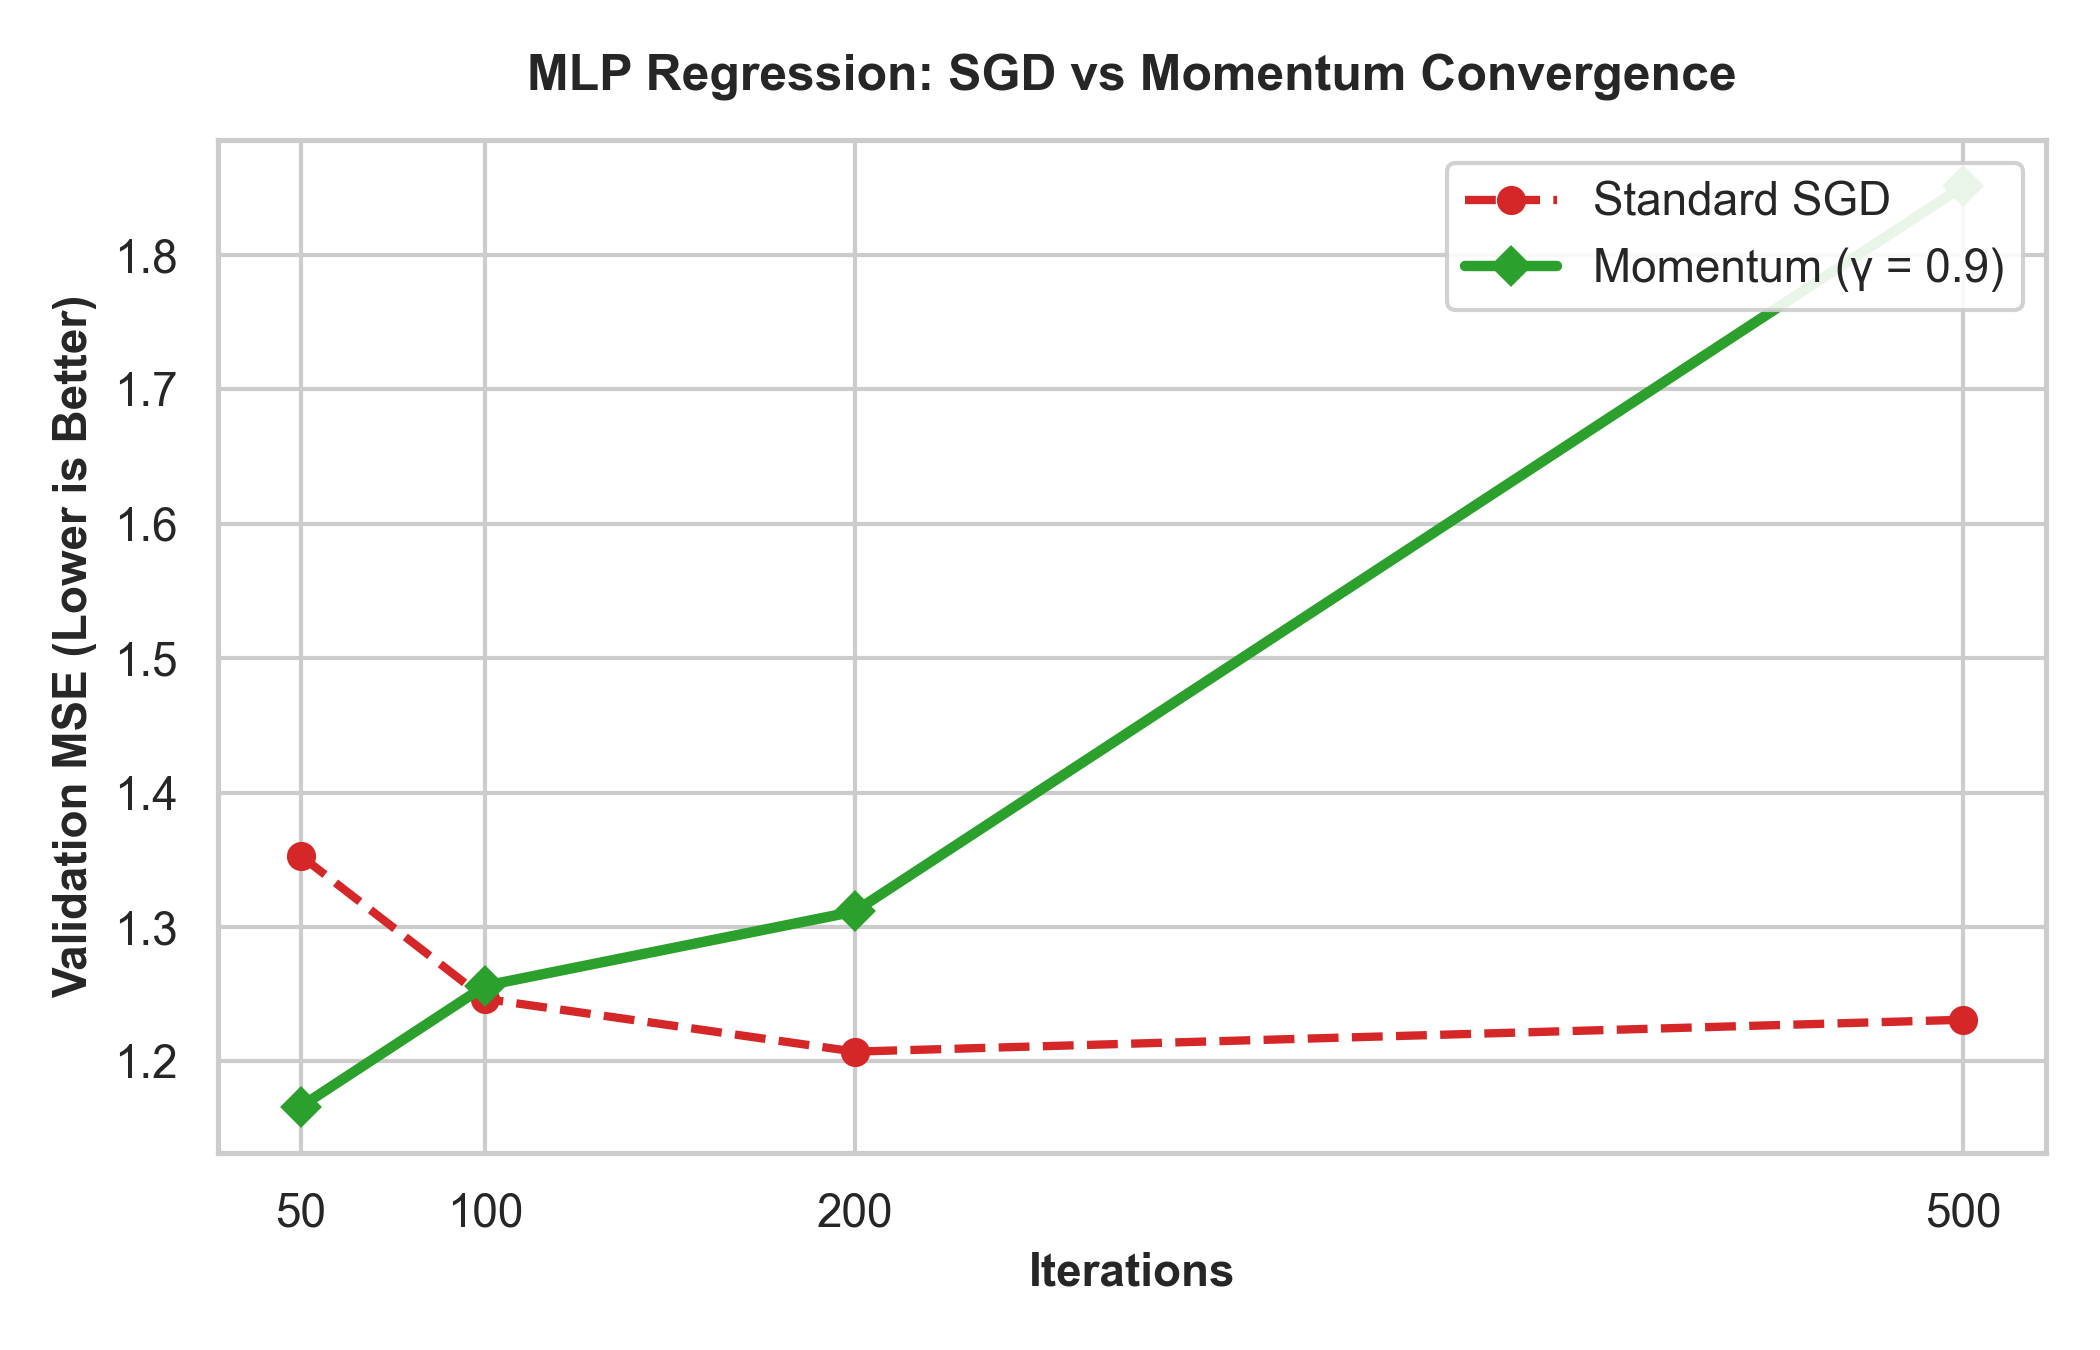
\includegraphics[width=0.96\linewidth]{mlp_reg_comparison.png}
        \caption{MLP Regression: SGD vs Momentum.}
        \label{fig:mlp_reg}
    \end{minipage}
    \vspace{-4mm}
\end{figure*}

\section{Methods}
Our MLP is built completely from scratch. The network supports arbitrary hidden layers. We initialise weights using a normal distribution scaled by $1 / \sqrt{I}$, where $I$ is the input dimension. Biases start at zero.

The forward pass runs layer-by-layer:
\begin{equation}
    \mathbf{A}^{(l)} = \mathbf{Z}^{(l-1)}\mathbf{W}^{(l)\top} + \mathbf{b}^{(l)}
\end{equation}
\begin{equation}
    \mathbf{Z}^{(l)} = \sigma^{(l)}(\mathbf{A}^{(l)})
\end{equation}
where $\mathbf{Z}^{(0)} = \mathbf{X}$. We implemented ReLU and Sigmoid activations.

For training, backpropagation propagates errors backward using the chain rule. We optimise parameters using Mini-Batch Gradient Descent (batch size = 32). We shuffle the training indices before each iteration to keep the gradients fresh.

We implement two loss functions:
\begin{itemize}
    \setlength{\itemsep}{0pt}
    \setlength{\parskip}{0pt}
    \item \textbf{Mean Squared Error (MSE):} Used for regression.
    \item \textbf{Cross-Entropy (CE):} Used for classification. We add a tiny offset ($\epsilon = 10^{-9}$) to prevent numerical blowups in the log.
\end{itemize}

For K-Means, we group features into $K$ clusters. We initialise centroids by grabbing random points from the data. Points are assigned to the nearest centroid using Euclidean distance. Centroids are updated as the mean of their assigned points. Empty clusters are resolved by selecting a random data point as the new centroid.
For classification, we assign a label to each centroid by majority vote of the true labels in its cluster. A new test point gets the label of its nearest cluster center.

\section{Experimental Setup}
We evaluate classification using Accuracy and Macro F1 score. Accuracy measures the percentage of correct predictions. However, because of the class imbalance, accuracy alone is misleading. Macro F1 calculates the F1 score for each class individually and averages them. This metric is much more sensitive to how well we predict the rare High class. For regression, we evaluate the addiction score predictions using Mean Squared Error (MSE). All models are trained on the 1,280 split training samples and evaluated on the 320 validation samples. All hyperparameter tuning and comparisons were performed on the validation split. The results reported in this milestone therefore correspond to validation performance.

\section{Hyperparameter Tuning}
We tuned the models systematically to find the best configurations. For K-Means, we swept $K$ from 1 to 20. For MLP Classification, we tuned standard SGD against our Momentum implementation ($\gamma = 0.9$) at a learning rate of $lr=0.01$ across iterations $\in [50, 500]$. For MLP Regression, we tuned standard SGD against Momentum at a learning rate of $lr=0.001$ across iterations $\in [50, 500]$.

\section{Results}
Our experiments produced the following results (summarised in Table 1 and visualised in Figures 1, 2, and 3):
\begin{itemize}
    \setlength{\itemsep}{0pt}
    \setlength{\parskip}{0pt}
    \item K-Means classification peaked at $K=5$, reaching 73.12\% accuracy (Macro F1 = 0.4172). However, $K=18$ gave 70.94\% accuracy but a much higher Macro F1 score of 0.5943.
    \item MLP classification with Momentum reached 75.94\% accuracy at just 100 iterations. Standard SGD required 500 iterations to reach that same level.
    \item MLP regression with standard SGD converged to an MSE of 1.1732 at 200 iterations. Momentum was faster initially, getting 1.2218 MSE at 50 iterations, but it overshot and diverged at higher iterations, rising to 2.0752 MSE.
\end{itemize}

\begin{table}[htbp]
\centering
\resizebox{0.95\columnwidth}{!}{%
\begin{tabular}{lll}
\toprule
Task & Model (Parameters) & Performance \\
\midrule
Classification & K-Means ($K=5$) & Acc: 73.12\%, F1: 0.4172 \\
Classification & K-Means ($K=18$) & Acc: 70.94\%, F1: 0.5943 \\
Classification & MLP + Momentum (iter=100) & Acc: 75.94\%, F1: 0.4556 \\
Regression & MLP + SGD (iter=200) & MSE: 1.1732 \\
\bottomrule
\end{tabular}%
}
\caption{Summary of final validation results}
\vspace{-4mm}
\end{table}

\section{Extensions}
We implemented three key extensions to improve our model:
\begin{enumerate}
    \setlength{\itemsep}{0pt}
    \setlength{\parskip}{0pt}
    \item \textbf{Momentum Optimiser (Lecture 9):} We added inertia to parameters using:
    \begin{equation}
        \mathbf{v}^{(l)} \leftarrow \gamma \mathbf{v}^{(l)} + \eta \nabla R(\mathbf{W}^{(l)})
    \end{equation}
    \begin{equation}
        \mathbf{W}^{(l)} \leftarrow \mathbf{W}^{(l)} - \mathbf{v}^{(l)}
    \end{equation}
    where $\gamma = 0.9$ and $\eta$ is the learning rate. We do the same for the biases. This helped classification speed up by 5x.
    \item \textbf{Cross-Entropy from Scratch:} We built multi-class cross-entropy and its gradient vectorisation from scratch:
    \begin{equation}
        \mathcal{L}_{\text{CE}} = -\frac{1}{N} \sum_{i=1}^N \sum_{c=1}^C y_{i}^{(c)} \ln(\hat{y}_{i}^{(c)} + \epsilon)
    \end{equation}
    The gradient w.r.t the predictions is:
    \begin{equation}
        \frac{\partial \mathcal{L}_{\text{CE}}}{\partial \hat{y}_{i}^{(c)}} = -\frac{y_{i}^{(c)}}{N(\hat{y}_{i}^{(c)} + \epsilon)}
    \end{equation}
    We fully vectorised this in NumPy using an $\epsilon = 10^{-9}$ for stability.
    \item \textbf{Deep MLP Architectures:} We tested a deep network configuration of $(D, 64, 32, C)$. It overfit the training set.
\end{enumerate}

\section{Runtime / Complexity Analysis}
We analysed the computational complexity of both algorithms. K-Means has a training complexity of $O(t \cdot N \cdot K \cdot D)$ where $t$ is iterations, $N$ is samples, $K$ is clusters, and $D$ is features. In practice, K-Means is extremely fast, fitting in 0.005 seconds on our system. MLP training complexity per iteration is $O(N \cdot \sum_{l=1}^L M_{l-1} \cdot M_l)$ where $M_l$ is the hidden dimension of layer $l$. Backpropagation is more expensive but still highly efficient, taking about 0.12 seconds for 100 iterations.

\section{Discussion}
Our results show some fascinating behaviors:
\begin{itemize}
    \setlength{\itemsep}{0pt}
    \setlength{\parskip}{0pt}
    \item \textbf{K-Means Class Imbalance Trade-off:} Why did K-Means get a higher Macro F1 at $K=18$ than $K=5$? Since Class 2 represents only 3.2\% of our dataset, a small $K$ creates large clusters where Class 2 is always outvoted during centroid labelling. When we increase $K$ to 18, clusters become smaller and more specialised. Some clusters capture only Class 2 samples, allowing those centroids to get the High label, which boosts our Macro F1 score.
    \item \textbf{Momentum Optimisation:} In classification, Momentum acted as a massive accelerator. By adding the moving average of gradients, it dampens oscillations in narrow valleys, speeding up training by 5x.
    \item \textbf{Momentum Overshooting in Regression:} In regression, Momentum worked well at first but diverged at 200+ iterations. This is because the accumulated velocity (inertia) pushed the weights past the narrow local minimum of the quadratic MSE loss. This is a classic limitation from Lecture 9!
\end{itemize}

\section{Limitations}
Our work has a few limitations:
\begin{itemize}
    \setlength{\itemsep}{0pt}
    \setlength{\parskip}{0pt}
    \item \textbf{Grid Resolution:} Our hyperparameter sweeps used a coarse grid (only testing 50, 100, 200, 500 iterations). A finer search might find better parameters.
    \item \textbf{Data Split Sensitivity:} We used a single 80/20 split. Our results might change slightly depending on the random seed of the split.
    \item \textbf{No Cross-Validation:} Due to the class imbalance, K-Fold cross-validation would be much more robust to ensure minority classes are represented in every fold.
    \item \textbf{Momentum Divergence:} Our momentum implementation lacks a learning rate decay schedule, making it prone to overshooting in regression tasks.
\end{itemize}

\section{Conclusion}
We successfully implemented K-Means and a multi-layer MLP from scratch. The supervised MLP classifier outperformed the unsupervised K-Means model (75.94\% vs 73.12\%) because it optimises directly for class boundaries. Adding momentum dramatically speeded up convergence in classification but proved unstable in regression due to overshooting. Overall, parametric neural nets are highly effective, but require careful tuning.

\end{document}
